\documentclass[letterpaper,11pt]{article}

\usepackage{pdfpages}
\usepackage[utf8]{inputenc}
\usepackage[spanish,mexico]{babel}
\usepackage{graphicx}
\usepackage{amsmath}
\usepackage{amsthm}
\usepackage{svg}
\usepackage{amsfonts}
\usepackage{subcaption}
\usepackage[margin=1.5cm,
vmargin={1cm,0.3cm},
includefoot]{geometry}
\usepackage{fancyhdr}
\pagestyle{fancy}
\renewcommand{\headrulewidth}{0.4pt}
\renewcommand{\footrulewidth}{0.4pt}


\begin{document}
	\setlength{\unitlength}{1cm}
	\thispagestyle{empty}
	\begin{picture}(19,3)
	\put(-0.5,1.2){
\includegraphics[scale=.20]{unam1.png}}
	\put(16,1){
\includegraphics[scale=.29]{fciencias1.png}}
	\end{picture}

\begin{center}
\vspace{-114pt}
\textbf{\large Estructuras de Datos}\\
\textbf{ Semestre 2020-2}\\
Prof. Alejandro Hernández Mora\\
Ayud. Pablo Camacho González  \\ 
Ayud. Lab. Luis Manuel Martínez Dámaso   \\
\rule{17cm}{0.3mm}\\
\textbf{Proyecto final}\\
\huge\textbf{Simulador Supermercado}\\[0.1cm]
\normalsize Kevin Ariel Merino Peña\footnote{317031326}\\
Armando Abraham Aquino Chapa\footnote{317058163}\\
\rule{17cm}{0.3mm}
\end{center}
%\vspace{-10pt}
%\begin{flushright}
%\vspace{-3pt}
%end{flushright}
\section*{Modelo del programa:}
\begin{figure}[htb]
	\centering
	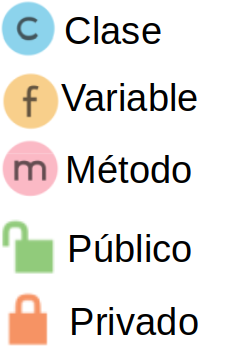
\includegraphics[scale=.24]{Simbologia.png}
	\caption{ Simbología para los diagramas de clases}
\end{figure}
A continuación se presentará una breve descripción del modelo del programa para la simulación del comportamiento de un supermercado con sus respectivos diagramas de clases.\\

\textbf{Main: }Contiene nuestro método principal que permite cumplir con el encapsulamiento y comportamiento del programa.
\begin{figure}[htb]
	\centering
	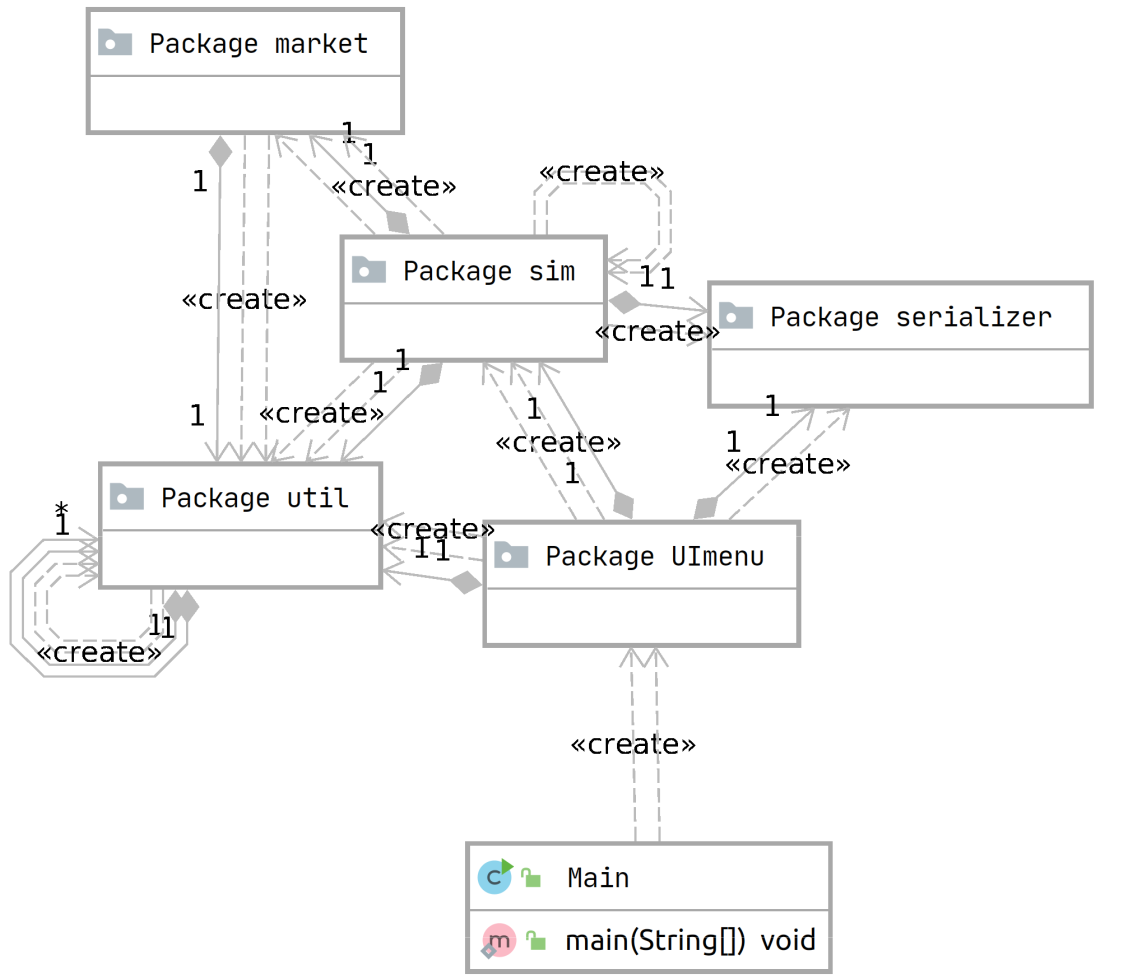
\includegraphics[scale=.29]{main_diagram.png}
\end{figure}

\textbf{Package UImenu: } Contiene nuestra clase \textit{Menu} dónde modelamos la interacción con la usuaria. Entre sus métodos principales se encuentran:

\begin{itemize}
	\item \textit{mainMenu: } Cómo su nombre lo indica se encarga de proveer dos opciones principales; "Modo Usuario", "Modo Administrativo" y por supuesto una opción para salir.
\end{itemize}
\begin{itemize}
	\item \textit{adminMenu:} Para uso administrativo del supermercado, en el cual podemos agregar, resurtir y ver el inventario de productos del mismo.
\end{itemize}
\begin{itemize}
	\item \textit{userMenu: } Aquí encontramos las funciones de las que podrá hacer uso cualquier persona, como hacer una simulación automática del supermercado, ó una simulación más personalizada ingresando el número de cajas rápidas y normales.
\end{itemize}
\begin{itemize}
	\item \textit{execPlot: } Se crean gráficas a partir del resultado de las simulaciones del supermercado para apreciar el comportamiento y rendimiento de las cajas del mismo para estudios posteriores.
\end{itemize}
\begin{figure}[htb]
	\centering
	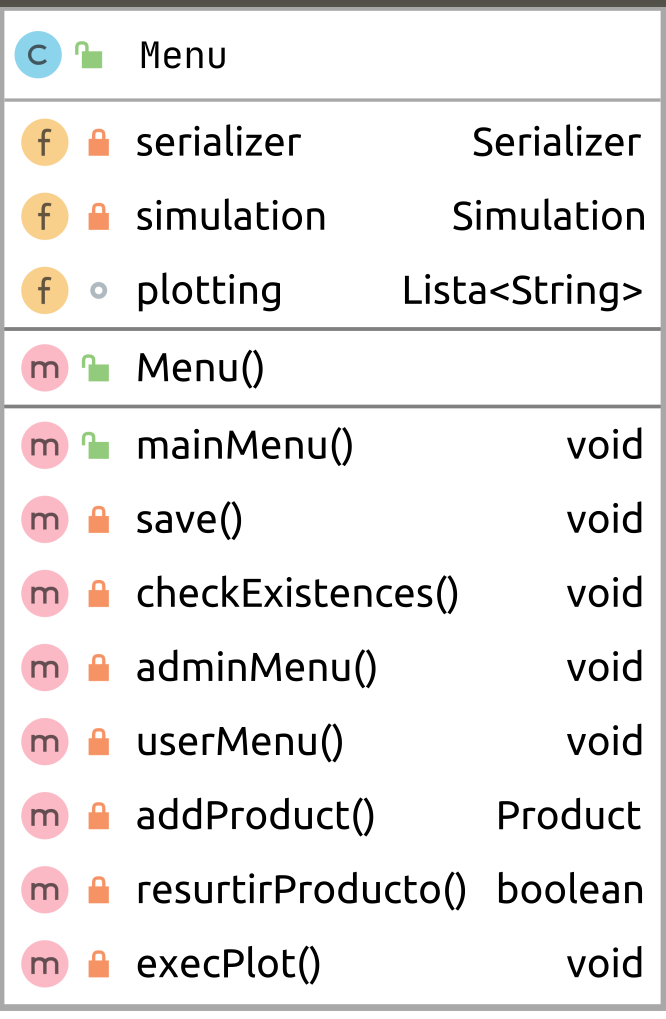
\includegraphics[scale=.29]{menu_diagram.png}
\end{figure}

\textbf{Package util: } En este paquete encontramos diversas clases, entre las cuales destacan las estructuras de datos utilizadas para modelar el supermercado y todo lo que lo engloba. Las estructuras de datos utilizadas son: \textit{Árbol Binario, de Búsqueda, Árbol AVL, Cola, Heap, Lista, Pila.}\\

También encontramos una clase llamada \textit{Utilities}, la cuál tiene la funcionalidad de contar con métodos auxiliares de la clase \textit{Menu } para que el programa sea persistente.\\
Por último encontramos dos clases llamadas \textit{Item, ItemBuilder} que generan productos aleatorios para el supermercado.\\
A continuación la representación en diagrama de clases.
\newpage
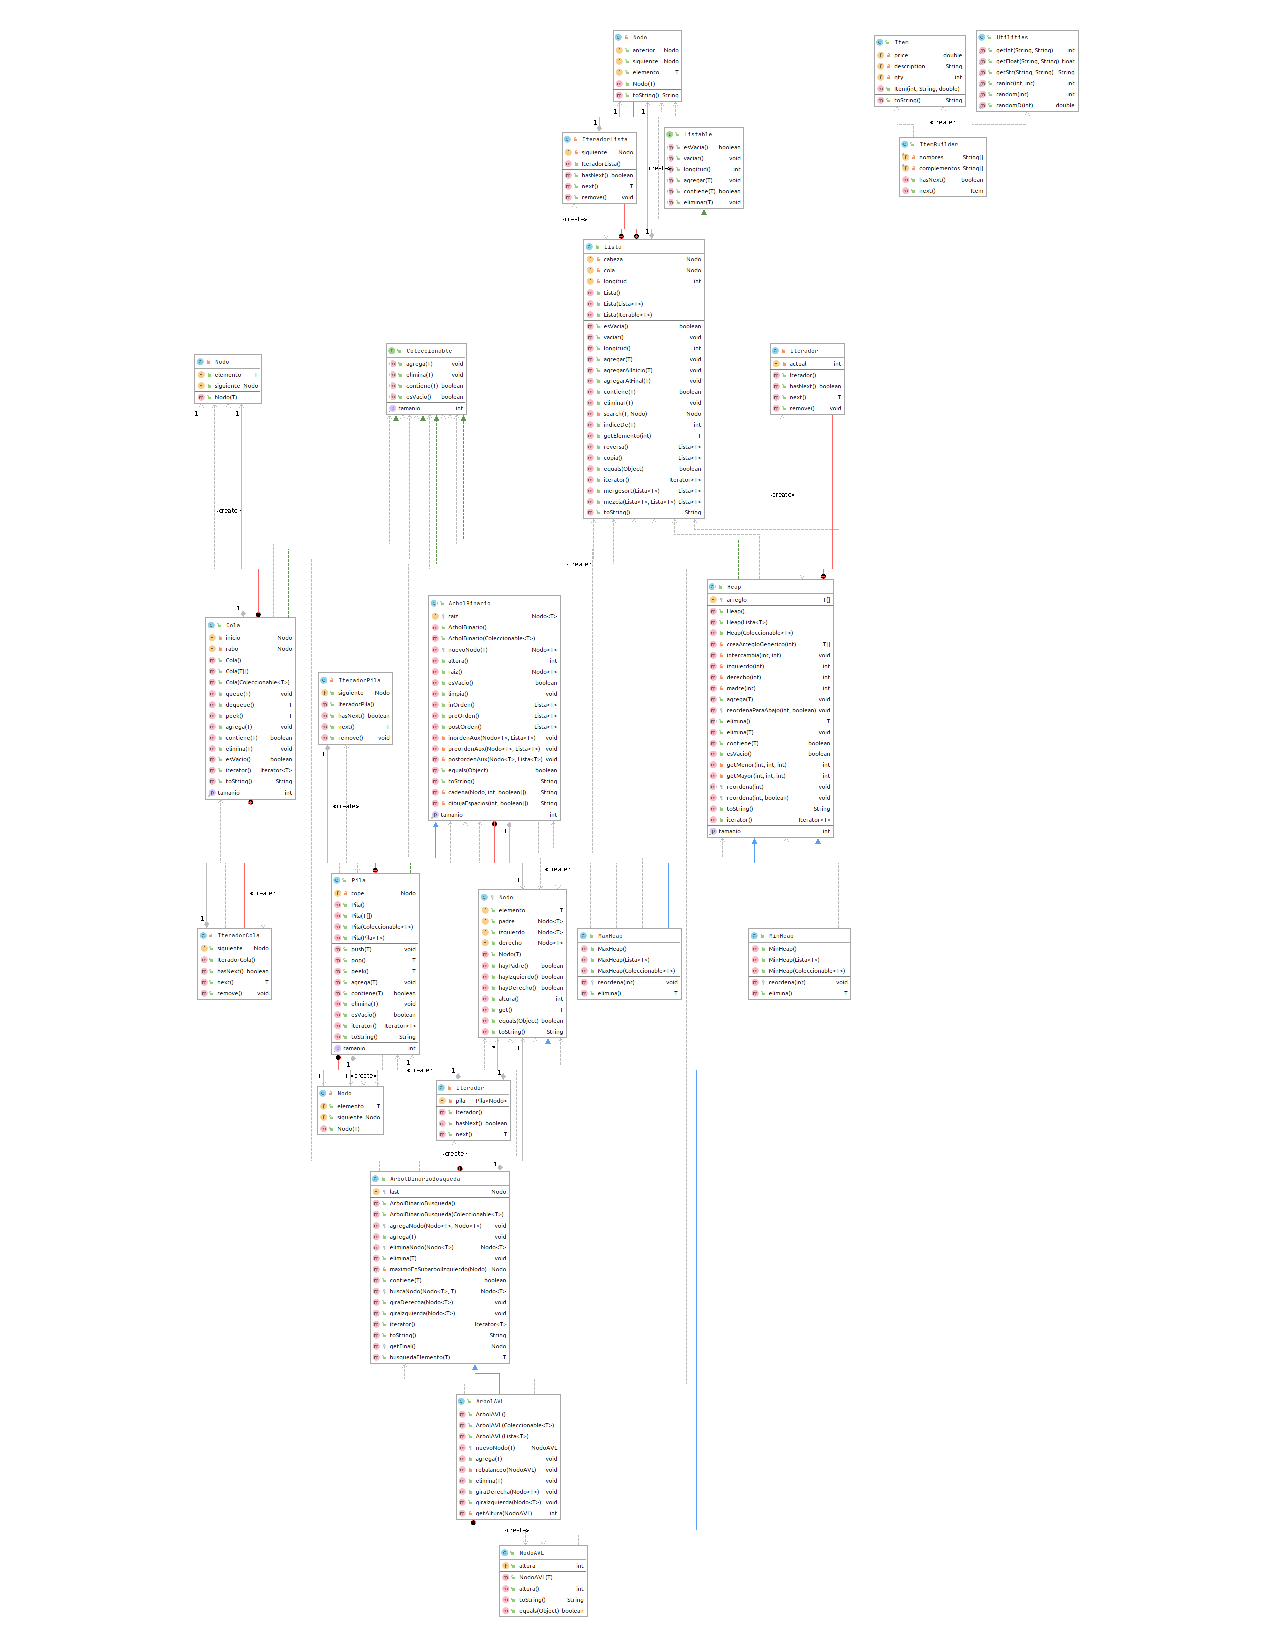
\includepdf[pages=-]{util}
\textbf{Package sim: } Este paquete contiene las clases necesarias que se encargan de gestionar la simulación del supermercado a través de hilos.
\begin{itemize}
	\item \textit{enterClient: } Simula el estado de un cliente en el supermercado, desde su ingreso a éste, formarse en alguna caja y pagar sus productos.
\end{itemize}
\begin{itemize}
	\item \textit{Simulation: } Engloba y ejecuta todos los aspectos necesarios para el comportamiento del supermercado. Un método a destacar es \textit{getReports} el cuál crea diversos directorios dónde se almacena el estado del supermercado después de las simulaciones, es decir, que productos tienen pocas existencias, los tickets generados de las diversas compras de los clientes, etc.
\end{itemize}
\begin{figure}[htb]
	\centering
	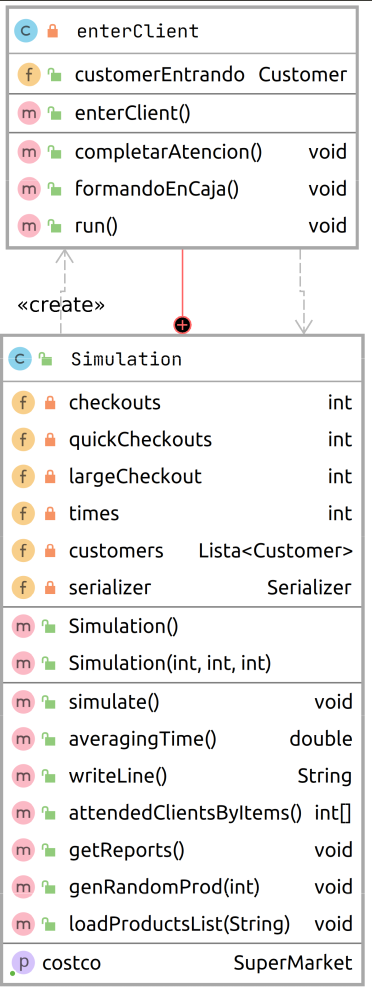
\includegraphics[scale=.37]{sim_diagram.png}
\end{figure}
\textbf{Package market: }
\begin{itemize}
	\item \textbf{Package admin: } Aquí se encuentran las clases para modelar los objetos que componen a un supermercado, tales como sus cajas (hay dos tipos: normal y rápida), sus productos (los cuales poseen un ID generado aleatoriamente, unidades en el inventario, nombre, precio) y un almacén dónde podemos consultar el inventario, modificar, ver los productos ue contiene, etc. 
\end{itemize}
\newpage
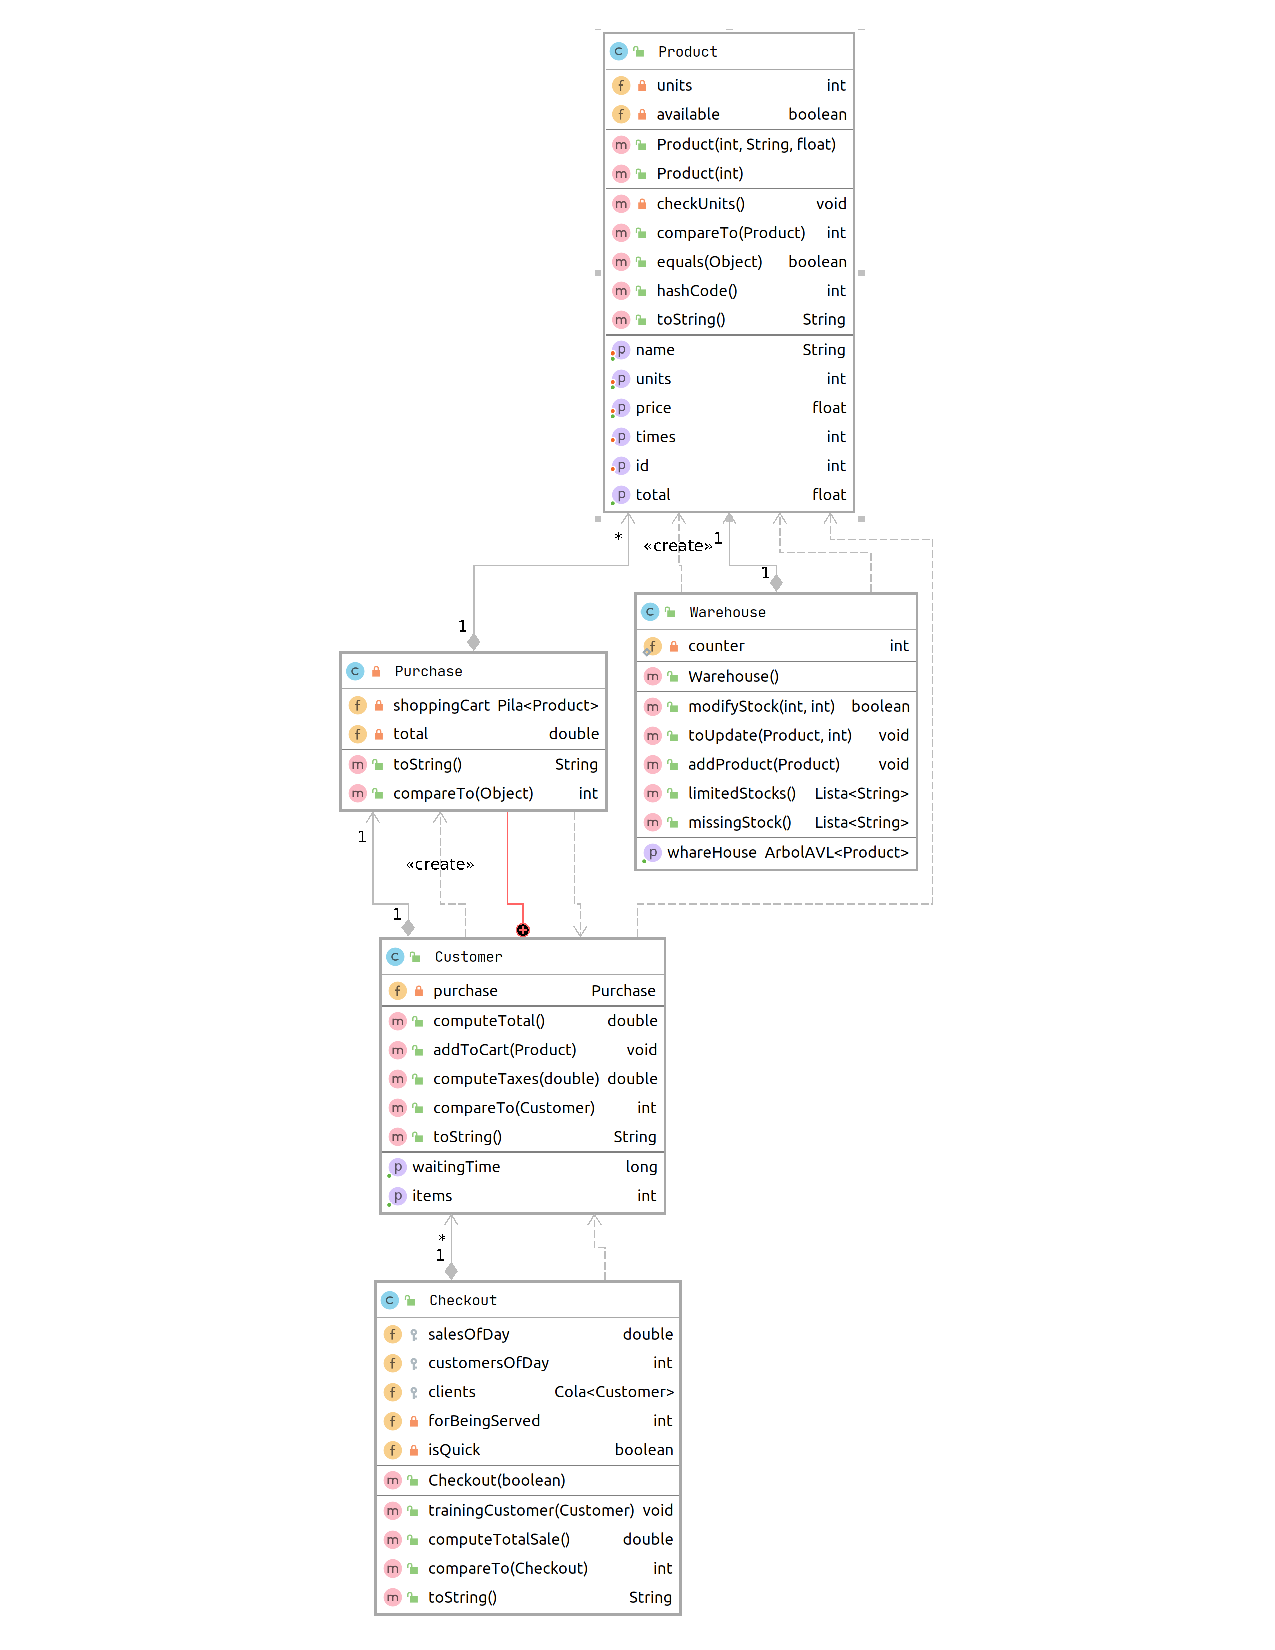
\includepdf[pages=-]{admin}
Por último tenemos la clase \textit{Supermaket: } que permite relacionar del paquete \textit{admin} y le otorga una estructura al supermercado.
\begin{figure}[htb]
	\centering
	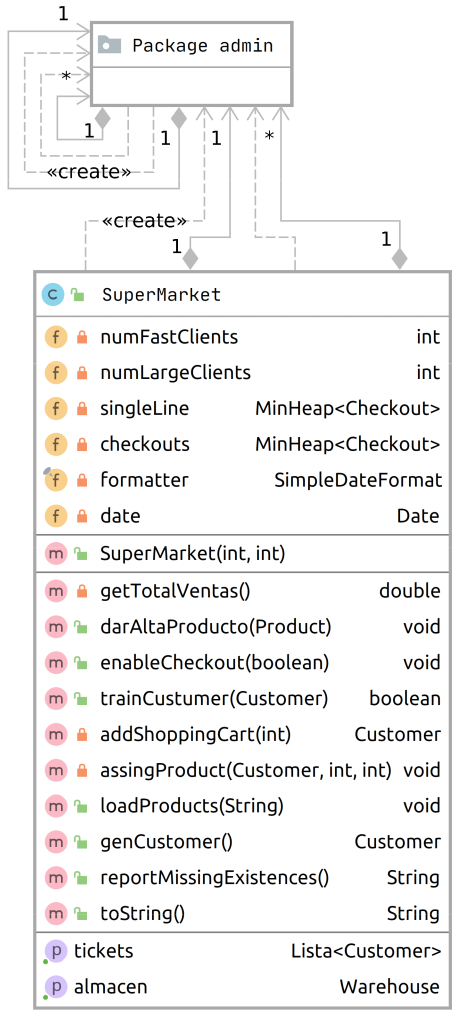
\includegraphics[scale=.39]{supermarket_diagram.png}
\end{figure}
\section*{Reporte de resultados:}

\end{document}
